\documentclass[
11pt, paper=a4,  listof=totocnumbered, % lists are also included in table of contents
numbers=noendperiod, % Don't add a period at the end of a chapter number
]{scrreprt}

    \usepackage{chngcntr}
    \counterwithout{footnote}{chapter}
    \counterwithout{figure}{chapter}
        \counterwithout{table}{chapter}
    
% ===============================
% IUBH Template für Seminar-, Bachelor-, and Master-works
% -------------------------------
% Authors; Ralf Kneuper, Jörg Sawatzki
% Maintainer: Paul Libbrecht

% Fix of Warning: Class scrreprt Warning: \float@addtolists detected!
% https://komascript.de/faq_float%40addtolist
\usepackage{scrhack}

% get custom bibliography style working without prepending [brackets]
\usepackage{natbib}
\setcitestyle{aysep={}} % remove comma as delimiter 

% breaks line at hyphens (resolves formatting issues in bibliography)
\usepackage[hyphens]{url}

\usepackage{txfonts} % Use a Times-new-roman open-source clone

% if you insist on Arial... then uncomment the following
%\usepackage{helvet}
%\renewcommand{\familydefault}{\sfdefault}

\usepackage{caption}
\usepackage{float}

\setkomafont{chapter}{\Large} 
\setkomafont{section}{\large}
\setkomafont{subsection}{\large} 

\usepackage[left=2cm,right=2cm,top=2cm,bottom=2cm]{geometry} % margins
\addtolength{\footskip}{-0.7cm}% foot larger by 0,7 cm  (Raises the page number)


\usepackage[onehalfspacing]{setspace} % line space 1,5

\setlength{\parindent}{6pt} % Indent at start of paragraphs  6pt

\usepackage[utf8]{inputenc} %UTF-8 to encode many characters => for many characters, you can just input the character and avoid a macro

\usepackage[english]{babel} % english hyphenations
%\usepackage[T1]{fontenc} %wichtig für Trennung von Wörtern mit Umlauten
\usepackage{microtype} % align margins

\usepackage{graphicx} % import graphics
\usepackage{placeins}% places the graphics within text

% Abbreviation's directory
% printonlyused - only if used
% withpage - the first occurrence's page number is listed too
\usepackage[withpage]{acronym}

\usepackage[hidelinks]{hyperref} %https://tex.stackexchange.com/questions/823/remove-ugly-borders-around-clickable-cross-references-and-hyperlinks

\usepackage{datetime}
\newdateformat{germandate}{\THEDAY. \THEMONTH. \THEYEAR}

\usepackage{listings}
%\lstset{numbers=left, numberstyle=\tiny, numbersep=5pt}
\lstset{language=Python}

\begin{document}
%TITELBLATT:!!!!!!!!!!!!!!!!!!!!!!!!!!!!!!!!!!!!!!!!!!!!!!!!!!!!!!!!!!!!!!!!!!!!!!!!!!!!!!!!!!!!!!!!!!!!!

\label{titlePage}
\begin{figure}[h]
\centering
\advance\leftskip--2cm

\includegraphics[width=0.50\textwidth]{pics/logo.pdf}
\end{figure}
\FloatBarrier

\begin{Large} 
\begin{center}

\end{center}
\end{Large} 

\vspace*{5mm}

\begin{large} 
\begin{center}
University of Applied Science - Online
\end{center}
\end{large} 

\begin{large} 
\begin{center}
Master: Data Science
\end{center}
\end{large}

\vspace*{15mm}

\begin{Large} 
\begin{center}
\textbf{Programmieren in Python}
\end{center}
\end{Large}

\vspace*{15mm}

\begin{large} 
\begin{center}
	Tim Willkens
\end{center}
\end{large} 

\vspace*{-6mm}

\begin{large} 
\begin{center}
Matrikelnummer: IU14073577
\end{center}
\end{large} 

%\vspace*{-6mm}

%\begin{large} 
%\begin{center}
%\end{center}
%\end{large} 

\vspace*{-6mm}

\begin{large} 
\begin{center}
Eiergäßle 11 \linebreak
89160 Dornstadt.
\end{center}
\end{large} 

\vspace*{5mm}

\begin{large} 
\begin{center}
Advisor: Dr. Prof. Thomas Kopsch
\end{center}
\end{large} 


\vspace*{-6mm}

\begin{large} 
\begin{center}
Delivery date: \germandate\today
\end{center}
\end{large} 


\pagestyle{empty} % no page numbering on the cover



\renewcommand{\thechapter}{\Roman{chapter}}

\pagestyle{plain}

\pagenumbering{Roman} %the intro is counted with roman numbers
\setcounter{page}{2} %starting with page 2 (page 1 is the titel)

% --- too detailed for a seminar but otherwise useful
%\chapter{Blocking notice (optional)}

Useful if this document contains information that should prevent redistribution.
%\chapter{Acknoowledgements (optional)}

Thanks to....
%\chapter{Abstract}



\tableofcontents %table of contents
\listoffigures %List of figures
\listoftables %list of tables

%% Abbreviations list
\renewcommand\refname{Abbreviations} \chapter{Abbreviations}
% The abbreviations list should contain all abbreviations that are not common-knowledge.
\begin{acronym}[NMWC] % the longest abbreviation here (for layout)
    \setlength {\itemsep}{-\parsep} % geringerer Zeilenabstand    	 

    \acro{AFL}{American Fuzzy Lop}
    \acro{API}{Application Programming Interface}
    \acro{BIOS}{Basic Input/Output System}
    \acro{Brick}{Binary Run-time Integer Based Vulnerability Checker}
    \acro{CaaS}{Container as a Service}
    \acro{CAB}{Change Advisory Board}
    \acro{CE}{Community Edition}
    \acro{CI}{Continuous Integration}
    \acro{CLI}{Command Line Interface}
    \acro{CNCF}{Cloud Native Computing Foundation}
%    \acro{CPU}{Central Processing Unit}
    \acro{CRED}{C Range Error Detector}
    \acro{Dev}{Development, the development team}
\end{acronym}

% Acronyms should be made hyperreffed the first time they appear in text with
% \ac{CI}  

\renewcommand{\thechapter}{\arabic{chapter}} %Count chapters with arabic numbers and not roman numbers
\setcounter{chapter}{0} %Reset chapter counter
\pagenumbering{arabic}

\chapter{Introduction}

Python, benannt nach der britischen Komikertruppe Monty Python, hat sich in den vergangenen Jahren zu einem Schwergewicht unter den Programmiersprachen entwickelt, \cite{Steyer:2018}.
Sie unterstützt sowohl die objektorientierte, die prozedurale sowie die funktionale Programmierung, \cite{Häberlein:2024}. Python wurde mit dem Ziel zur Förderung eines gut lesbaren sowie knappen Programmierstiels entwickelt, \cite{Steyer:2018}. 
Im Gegensatz zu compelierten Sprachen wie Java oder C \# ist zählt Python zu den interpretierten Programmiersprachen und kann somit ohne weiteres auf einem anderen Betriebssystem ausgeführt werden, \cite{Häberlein:2024}. \\
Aufgrund der Vielzahl an Bibliotheken wie NumPy, Pandas, SciKit-Learn und MatplotLib hat Python Einzug als Standardprogramm in die Wissenschaften, die Data Science und des maschinellen Lernen erhalten, \cite{VanderPlas:2023}. \\
In der nachfolgenden Arbeit wird auf grundlegenden Techniken zur Programmentwicklung mittels Python eingegangen. Beginnend mit der Objektorientierten Programmierung, welche sich als bewährte Methode zur Erstellung komplexer Softwaresysteme erwiesen hat, \cite{Lahres:2021}.\\
Weiter werden Teile der Datenverarbeitung mit Pandas sowie dem Arbeiten mit Datenbanken behandelt. Pandas ist eine Open Source Bibliothek welche vorallem im Data Science Umfeld zum Einsatz kommt, \cite{Nelli:2023}. Eng hiermit verbunden ist das Thema des maschinellen Lernens welches ebenfalls kurz behandelt wird. Hierzu wird Scikit-Learn Bibilothek verwendet, welche effiziente Implementierungen vieler Machine Learning Algorithmen beinhaltet, \cite{Geron:2022}. Die Visualisierung erfolgt mittels \textit{bokeh}. Bokeh ist eine Python-Bibliothek zur Erstellung interaktiver Visualisierungen für moderne Webbrowser, \cite{Boekeh}\\ 
Das erzeugte Programm soll nach gängigen Entwicklungsstandards. Dies beinhaltet unter anderem auch eine klare Dokumentation. Hierzu werden sogenannte \textit{docstrings}  \textit{unittests} verwendet. Ein \textit{docstring} ist ein String-Literal welcher direkt im Sourcecode eingefügt wird, \cite{Pajankar:2022}. Ein \textit{unittest} ist eine Testmethode bei der einzelne Komponenten eines Programms unabhängig voneinander getestet werden, \cite{Pajankar:2022}. \\
Die Versionskontrolle wird über \textit{Git} verwaltet. Speziell in großen Software-Projekten bietet Git den Entwicklern die Erstellung und Pflege der Versionskontrolle und erstellt im Vergleich zu CVS per se keine kanonische Kopie der Codebasis. Alle Kopien sind Arbeitskopien und können lokal verändert werden ohne mit einem Server verbunden zu sein \cite{Russell:2019}

\chapter{Objektorientierte Programmierung}\label{Objektorientierte Programmierung}

Die objektorientierte Programmierung hat seine Anfänge in den 1970er Jahren und setzte sich in den 1990er Jahren mit der Einführung von Java durch, \cite{Steyer:2018}. Sie unterstützt komplexe Softwareentwicklung dabei, Software einfacher erweiterbar, besser testbar und besser wartbar zu machen, \cite{Lahres:2021}. Als wesentliche Grundelemente der OOP gelten, \cite{Lahres:2021}


\begin{itemize}
	\itemsep0pt
	\item Unterstützung von \textbf{Vererbungsmechanismen}: \\
	Attribute, Methoden und Ereignisse werden von der Basisklasse auf die abgeleitete Klasse übertragen. Dies ermöglicht die Wiederverwendung von Code und die Erweiterung der Funktionalität.
	\item Unterstützung von \textbf{Datenkapselung}: \\
	Ist ein Konzept, Daten und Informationen vor dem direkten Zugriff von außen zu verbergen. Es ermöglicht die Kontrolle über den Zugriff auf die internen Datenstrukturen eines Objekts und erfolgt über definierte Schnittstellen.
	\item Unterstützung von \textbf{Polymorphie}: \\
	Ermöglicht, dass ein Bezeichner abhängig von seiner Verwendung Objekte unterschiedlichen Datentyps annimmt. Dies bedeutet, dass eine einzige Schnittstelle oder Methode verschiedene Implementierungen haben kann.
\end{itemize}

Objektorientierte Programmierung (OOP) ist somit ein Programmierparadigma, dass auf dem Konzept von "Objekten" basiert die Datenstrukturen enthalten und Verhaltensweisen (Methoden) definieren. Diese Objekte sind Instanzen von Klassen, die als Blaupausen für Objekte dienen. 

\section{Klassen}
Eine Klasse ist eine Vorlage oder ein Bauplan für die Erstellung von Objekten. Sie definiert die Attribute und Methoden, die ein Objekt haben wird. Ein Attribut ist eine Eigenschaft oder ein Merkmal, das ein Objekt hat, während eine Methode eine Funktion ist, die ein Objekt ausführen kann, \cite{Steyer:2018}. Klassen werden durch das Schlüsselwort \textit{class} definiert. 

\begin{lstlisting}[caption={class Data}, captionpos=b, label={lst:class data}]
class Data():
  def __init__(self, datapath):
    try:
      self.datapath = datapath
      self.df = pd.read_csv(datapath)
    except FileNotFoundError:
      print(sys.exc_info())
    cols = self.df.columns
    for i in cols:
      self.__dict__[i] = self.df[i]
    self.dfSortByX = self.df.sort_values(['x'])
\end{lstlisting}

\section{Methoden und Vererbung}
Die Klasse \textit{Data} hat eine Methode \textit{\_\_init\_\_}, welche den Parameter \textit{datapath} entgegen nimmt und versucht, eine CSV-Datei von diesem Pfad zu lesen und in ein DataFrame zu konvertieren. Wird die Datei nicht gefunden, wird eine Fehlermeldung ausgegeben. Die Methode \textit{\_\_init\_\_} initialisiert auch andere Attribute der Klasse, wie df und \textit{dfSortByX}.

Allgemein ist die \textit{\_\_init\_\_} Methode in Python ist eine spezielle Methode, die automatisch aufgerufen wird, wenn eine Instanz (ein Objekt) einer Klasse erstellt wird. Sie wird verwendet um die Attribute der Klasse zu initialisieren. Die \textit{self} Variable repräsentiert die Instanz der Klasse und wird verwendet um auf die Attribute und Methoden der Klasse zuzugreifen, \cite{Häberlein:2024}. \\

Vererbung ist ein Prinzip der OOP, dass es ermöglicht eine neue Klasse zu erstellen, welche die Attribute und Methoden einer bestehenden Klasse erbt. Die neue Klasse wird als "Unterklasse" oder "abgeleitete Klasse" bezeichnet, während die bestehende Klasse als "Oberklasse" oder "Basis-Klasse" bezeichnet wird, \cite{Steyer:2018}.
Die Klasse \textit{IdealFunctions} erbt von Data und fügt die Methode \textit{GetIdealFunctions} hinzu, die eine ideale Funktion basierend auf einem Trainingsdatensatz berechnet. Anhand des kleinsten Fehler zwischen den Trainingsdaten und den Daten der Basisklasse gibt die Methode die Indizes der idealen Funktionen zurück.

\begin{lstlisting}[caption={class IdealFunctions}, captionpos=b, label={lst:class IdealFcns}]
class IdealFunctions(Data):
  def __init__(self, datapath):
    Data.__init__(self, datapath)
  def GetIdealFunctions(self, dfTrain:pd.DataFrame):
    ...
\end{lstlisting}

Die Klasse \textit{TestData} erbt ebenfalls von Data und enthält die Methode \textit{Segmentation}, die eine Segmetierungsfunktion für einen gegebenen Datensatz implementiert. Diese Methode ordnet Datenpunkte basierend auf einem Schwellenwert \textit{threshold}, welche mit $\sqrt{2}$ initialisiert wird, einer Idealen Funktion zu.

\begin{lstlisting}[caption={class TestData}, captionpos=b, label={lst:class IdealFcns}]
class TestData(Data):
  def __init__(self, datapath):
    Data.__init__(self, datapath)
  def Segemtation(self, dataFrame:pd.DataFrame, threshold= np.sqrt(2))
    ...
\end{lstlisting}


%\chapter{Objektorientierte Programmierung}

Objektorientierte Programmierung (OOP) ist ein Programmierparadigma, das auf dem Konzept von "Objekten" basiert, die Datenstrukturen enthalten und Verhaltensweisen (Methoden) definieren. Diese Objekte sind Instanzen von Klassen, die als Blaupausen für Objekte dienen. Eine der Hauptfunktionen der OOP ist die Vererbung, ein Mechanismus, der es ermöglicht, Code zu teilen und zu wiederverwenden. In diesem Bericht werden wir diese Konzepte anhand eines Beispiels aus der Datenverarbeitung und Datenbankverwaltung erläutern.

\section{Klassen}
Eine Klasse ist eine Vorlage oder ein Bauplan für die Erstellung von Objekten. Sie definiert die Attribute und Methoden, die ein Objekt haben wird. Ein Attribut ist eine Eigenschaft oder ein Merkmal, das ein Objekt hat, während eine Methode eine Funktion ist, die ein Objekt ausführen kann.

Die \textit{\_\_init\_\_} Methode in Python ist eine spezielle Methode, die automatisch aufgerufen wird, wenn eine Instanz (ein Objekt) einer Klasse erstellt wird. Sie wird verwendet, um die Attribute der Klasse zu initialisieren. Die \textit{self} Variable repräsentiert die Instanz der Klasse und wird verwendet, um auf die Attribute und Methoden der Klasse zuzugreifen.

In unserem Beispiel haben wir eine Klasse Data, die eine Methode \textit{\_\_init\_\_} hat. Diese Methode nimmt einen Parameter datapath entgegen und versucht, eine CSV-Datei von diesem Pfad zu lesen und in ein DataFrame zu konvertieren. Wenn die Datei nicht gefunden wird, wird eine Fehlermeldung ausgegeben. Die Methode \textit{\_\_init\_\_} initialisiert auch andere Attribute der Klasse, wie df und \textit{dfSortByX}.\\

\begin{lstlisting}[caption={class Data}, label={lst:class data}]
class Data():
  def __init__(self, datapath):
    try:
      self.datapath = datapath
      self.df = pd.read_csv(datapath)
    except FileNotFoundError:
      print(sys.exc_info())
    cols = self.df.columns
    for i in cols:
      self.__dict__[i] = self.df[i]
    self.dfSortByX = self.df.sort_values(['x'])
\end{lstlisting}

\section{Vererbung}
Vererbung ist ein Prinzip der OOP, das es ermöglicht, eine neue Klasse zu erstellen, die die Attribute und Methoden einer bestehenden Klasse erbt. Die neue Klasse wird als "Unterklasse" oder "abgeleitete Klasse" bezeichnet, während die bestehende Klasse als "Oberklasse" oder "Basis-Klasse" bezeichnet wird.

In unserem Beispiel haben wir zwei Klassen \textit{IdealFunctions} und \textit{TestData}, die von der Klasse Data erben. Sie erben alle Attribute und Methoden von Data und definieren zusätzliche Methoden.

Die \textit{self} Variable wird verwendet, um auf die Attribute und Methoden der Klasse zuzugreifen, die von der Oberklasse geerbt wurden. Zum Beispiel, in der \textit{\_\_init\_\_} Methode der \textit{IdealFunctions} Klasse, rufen wir die \textit{\_\_init\_\_} Methode der Data Klasse auf, um die Attribute der Data Klasse zu initialisieren.

\begin{lstlisting}[caption={class Data}, label={lst:class IdealFcns}]
class IdealFunctions(Data):
  def __init__(self, datapath):
    Data.__init__(self, datapath)
\end{lstlisting}
\chapter{Python Bibliotheken}

Für Python gibt es Bibliotheken zum Laden von Daten, Visualisieren, Berechnen von Statistiken, Sprachverarbeitung, Bildverarbeitung usw. Dies gibt Data Scientists einen sehr umfangreichen Werkzeugkasten mit Funktionalität für allgemeine und besondere Einsatzgebiete, \cite{Mueller:2017}.
Numpy ist das Modul der Wahl, wenn man wissenschaftlich rechnen möchte und wird insbesondere für statistische Auswertungen, für Machine-Learning und allgemein für sehr aufwändige Berechnungen eingesetzt. Auf Numpy setzt unter Anderem auch TensorFlow, pandas, scipy, scikit-learn auf, \cite{Häberlein:2024}.

\section{Numpy}
NumericalPython, kurz NumPy, bietet Datenstrukturen und Algorithmen speziell für wissenschaftliche Anwendungen, \cite{McKinney:2023}. Grund hierfür ist, dass die Berechnung bei großen Daten-Arrays besonders effizient ist und somit schneller als normaler Python Code sein kann, \cite{McKinney:2023}. \\
Viele weitere Bibliotheken wie Pandas bauen auf NumPy auf, \cite{VanderPlas:2023}. Weitere Informationen der einzelnen Module können aus der NumPy Dokumentation entnommen werden, \cite{NumPy}

\section{Pandas}
 Pandas ist eine neuere Bibliothek und findet in der DataScience hohe Anwendung.  Sie bietet eine komfortable Schnittstelle zum speichern von Daten sowie eine Vielzahl an nützlicher Operationen. Die drei wichtigsten Datenstrukturen sind \textit{Series}, \textit{Index} und \textit{DataFrames}, \cite{VanderPlas:2023}.\\
 Ein DataFrame ist eine zweidimensionale, potenziell heterogene tabellarische Datenstruktur mit beschrifteten Achsen (Zeilen und Spalten). Diese entsprechen einem Zeilen- sowie Spaltenindex. Es kann als eine Art Container für Series-Objekte betrachtet werden, ähnlich wie ein Wörterbuch, das Spaltennamen als Schlüssel und Series-Objekte als Werte enthält. Ein DataFrame kann aus verschiedenen Datenquellen wie Listen, Dictionaries oder anderen DataFrames erstellt werden. Es bietet eine Vielzahl von Funktionen zur Datenmanipulation und -analyse und ist besonders nützlich für Aufgaben im Bereich der Datenanalyse. Pandas DataFrames können beispielsweise aus CSV-Dateien, Excel-Dateien oder SQL-Datenbanken eingelesen werden, \cite{VanderPlas:2023}. \\
 Beispielsweise kann ein Datensatz der Form 
 \begin{table}[H]
 	\small
 	\centering
 	\begin{tabular}{p{1.5cm}|p{1.5cm}|p{1.5cm}|p{1.5cm}|p{1.5cm}}
 		$x$ & $y_1$ & $y_2$ & $y_3$ & $y_4$ \\ \hline
 		-20.0 & 100.21 & -19.75 & 0.34 & 19.77 \\
 		-19.9 & 99.89 & -19.70 & 0.61 & 19.78 \\
 		-19.8 & 99.39 & -19.56 & 0.17 & 19.44 \\
 		-19.7 & 98.24 & -19.85 & 0.73 & 19.86 \\
 	\end{tabular}
 	\caption{Beispiel Panda DataFrame}
 	\label{tab:Pandas DF}
 \end{table}
 folgendermaßen
 \begin{lstlisting}[caption={Pandas Dataframe}, captionpos=b, label={lst:Dataframe}]
	data = 
	{
		'x': [-20.0, -19.9, -19.8, -19.7],
		'y1': [100.216064, 99.894684, 99.397385, 98.24446],
		'y2': [-19.757296, -19.70282, -19.564255, -19.858267],
		'y3': [0.3461139, 0.61786354, 0.1743704, 0.7310719],
		'y4': [19.776287, 19.789793, 19.441765, 19.869267]
	}
	df = pd.DataFrame(data)
 \end{lstlisting}
 in ein Dataframe geschrieben werden. Dieses DataFrame hat den Spaltenindex \textit{'x', 'y1', y2', 'y3', 'y4'}, abrufbar über \textit{df.columns}, sowie den Zeilenindex \textit{'0', '1', '2', '3'}, abrufbar über \textit{df.index}.\\
 
 In der Klasse \textit{Data} aus Kapitel \ref{lst:class data} wird mittels der Pandas Funktion
 \begin{lstlisting}
 	self.df = pd.read_csv(datapath)
 \end{lstlisting}
 eine .csv Datei eingelesen und als DataFrame gespeichert. 
 Weitere nützliche Funktionen sind die \textit{df.sort} Funktion
 \begin{lstlisting}
 	self.dfSortByX = self.df.sort_values(['x'])
 \end{lstlisting}
 welche das DataFrame anhand der x-Spalte sortiert.
 
 \section{Bokeh}
 Bokeh ist eine interaktive Datenvisualisierungsbibliothek für Python, die sich dadurch auszeichnet, umfassende interaktive Grafiken zu erstellen. Sie ist kompatibel mit Webtechnologien wie HTML, CSS und JavaScript und kann auf verschiedenen Plattformen wie Jupyter Notebook, JupyterLab, Flask und Django eingesetzt werden.
 Sie bietet eine breite Palette von Diagrammtypen, darunter Linien-, Streu-, Balken-, Flächen-, Histogramme- und zahlreiche weitere Diagramme. Bokeh zeichnet sich durch seine Schnelligkeit bei der Arbeit mit großen Datensätzen aus und ermöglicht es Nutzern, Grafiken anzupassen und interaktiv zu betrachten. 
 
Abbbildung \ref{fig:bokeh} dient beispielhaft für die Erstellung eines Plots mittels Bokeh. Diese wurde mit dem \textit{scatter}- Befehl erstellt und verarbeitet die \textit{x} und \textit{y} werte eines Pandas \textit{DataFrame}.
 \begin{figure}[h]
 	\centering
 	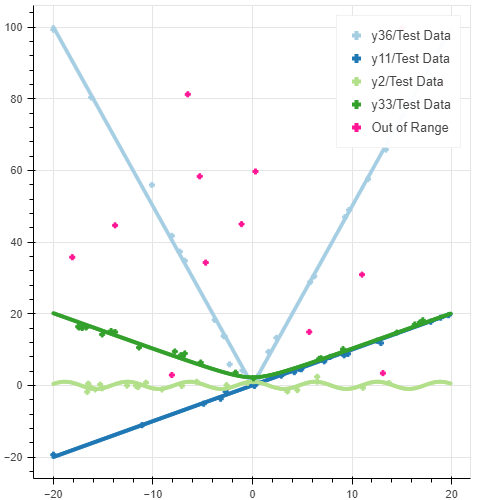
\includegraphics[width=8cm]{pics/bokeh_plot.png}
 	\caption{Beispiel eines Plots mit Bokeh }
 	\label{fig:bokeh}
 \end{figure} 
 
 \begin{lstlisting}[caption={Bsp.: Bokeh Scatter-Plot}, captionpos=b, label={lst:plot}]
 	ax.scatter(idFcnsDf['x'].values, idFcnsDf['y'].values,size=3,
 		color=colors[i])
 \end{lstlisting}
 
 Müssen mehrere Farben verwendet werden, bietet Bokeh eine breite Auswahl an Farbpaletten. Abbildung \ref{fig:bokeh} wurde mit der \textit{brewer paired} Farbpalette erstellt. 
 \begin{lstlisting}[caption={Bokeh Farb-Palette}, captionpos=b, label={lst:brewer color}]
 	colors = palettes.brewer['Paired'][4]   
 \end{lstlisting}
 
\chapter{Datenbanken}

Ein zentraler Bestandteil bei der Programmierung ist das arbeiten mit Daten und Dateien. Um mit großen und komplexen Datenmengen effizient und widerspruchsfrei zu arbeiten wird ein Verwaltungssystem benötigt. Dies führt zu Datenbankkonzepten wie SQL, \cite{Steyer:2018}.
Dabei ist SQL (Structured Query Language) ein internationaler Standard zum arbeiten mit Daten, aber keine Universalsprache wie etwa \textit{Java} oder \textit{C}, \cite{Taylor:2023}. Es wurde entwickelt um mit Relationalen Datenbanken zu arbeiten, welche Daten in Tabellenform organisieren sowie Beziehungen zwischen Tabellen herstellen können.

Python bietet Bibliotheken zum arbeiten mit SQL Datenbankkonzepten wie \textit{MySql}, \textit{SQLite} und weitere an.

Nachfolgend sind die wichtigsten schritte zum arbeiten einer SQLite - Datenbanken sowie der \textit{SQLAlchemy}- Bibliothek aufgeführt.
\begin{itemize}
	\itemsep0pt
	\item Verbinden mit der Datenbank \textit{dbName} über \textit{conncet()}
	\begin{lstlisting}
my_db = sqlite3.connect(dbName)
	\end{lstlisting}
	\item Erstellen eines \textit{Engine}- Objekts mit dem Pfad zur Datenbank 
	\begin{lstlisting}
engine = db.create_engine(databasePath)
	\end{lstlisting}
	\item Speichern eines DataFrames in eine Datenbank
	\begin{lstlisting}
dataFrame.to_sql(dbTableName, con=engine, if_exists='replace', index = False)
	\end{lstlisting}
	\item Lesen von Daten aus der Datenbank und in einem DataFrame zur Verfügung stellen
	\begin{lstlisting}
tableDF = pd.read_sql_table(self.dbTableName, engine, columns = None)
	\end{lstlisting}
	\item Verbindung zur Datenbank beenden (um ressourcen zu schonen)
	\begin{lstlisting}
engine.dispose()
my_db.close()
	\end{lstlisting}
	
\end{itemize}
\chapter{Versionskontrolle mit Git}

Speziell in großen und komplexen Software-Projekten ist eine gute Versionskontrolle des zu entwickelnden Codes unabdingbar.
Hierfür hat sich Git in den letzten Jahren als Standard entwickelt. Git ist besonders leistungsfähiges und flexibles Versionskontrollwerkzeug mit geringem Aufwand, dass die Entwicklung im Team immens vereinfacht, \cite{Loeliger:2012}.

Hierbei ermöglicht Git das arbeiten in sogenannten \textit{Repositories}. Dies sind einfache Datenbanken, welche alle nötigen Informationen enthält, die für die Aufbewahrung und Verwaltung der Revisionen und des Verlaufs eines Projekts erforderlich sind, \cite{Loeliger:2012}. Dabei werden zwischen lokalen und remote Repositories unterschieden. Auf das remote Repository kann das gesamte Entwicklungsteam zurückgreifen und enthält den aktuellsten Stand der zu entwickelnden Software. Die Entwicklung hingegen erfolgt meistens auf lokalen Repositories, auf welche nur einzelne Entwickler, bzw kleine Entwicklungsteams zugriff haben.

Über den \textbf{clone}- Befehl kann ein Klon des remote Repository im lokalen Repository erzeugt werden.
Weitere wichtige Befehle zum arbeiten mit Repositories sind:
\begin{itemize}
	\item  \textbf{pull}:
	Änderungen aus einem (remote) Repository in das (lokale) Repository übernehmen.
	\item  \textbf{push}:
	Änderungen des (lokalen) Repository in das (remote) Repository einfügen.
\end{itemize}

Zentraler Bestandteil der Versions-Kontrolle sind sogenannte \textit{commits}. Werden Änderungen am Code bzw. am Software-Projekt vorgenommen, dann kann einen neue Version über den \textbf{commit}- Befehl erstellt werden. Hierbei werden auch nützliche Informationen wie der Author, Kommentare und eine Commit-Id, sowie alle Änderungen gespeichert. Somit ist zu jedem Zeitpunkt möglich diesen Stand wiederherzustellen.

Weiter ist es möglich, dass mehrere Entwickler parallel an der Entwicklung arbeiten. Hierzu bietet Git das arbeiten in sogenannten Branches. Eine Branche ist eine Abzweigung eines bestimmten Commits und somit einem bestimmten Stand. Diese werden über den \textbf{branch}- Befehl erzeugt. Weitere wichtige Befehle zum Arbeiten mit Branches sind:
\begin{itemize}
	\item  \textbf{chekout}:
	Wechsel in eine andere Branch.
	\item  \textbf{merge}:
	Zwei Branches zu einer Branch zusammenführen.
\end{itemize}  

In Abbildung \ref{fig:Git} ist beispielhaft ein Git-Projekt dargestellt. Hier sind vier Branches (testing, dev, master, Stabel) sowie mehrere Commits (A - Z) zu sehen.

\begin{figure}[h]
	\centering
	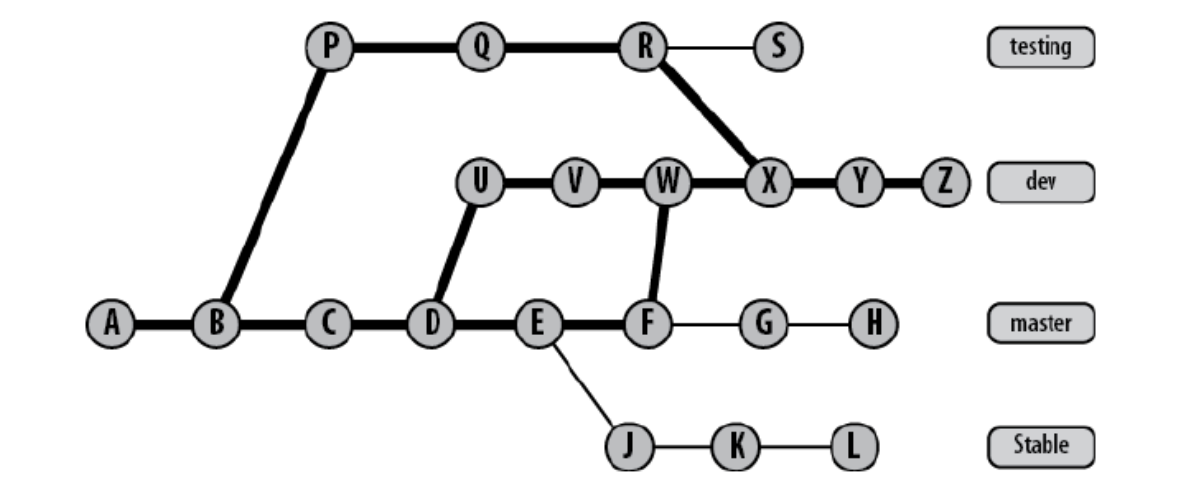
\includegraphics[width=8cm]{pics/Git.png}
	\caption{Branches und Commits, \cite{Loeliger:2012}}
	\label{fig:Git}
\end{figure}  
\chapter{Zusammenfassung}


Python ist eine moderne Programmiersprache, die vollständig auf die objektorientierte Programmierung (OOP) setzt, um die Modellierung komplexer Systeme zu erleichtern sowie leicht verständlich ist. Die OOP in Python orientiert sich an der realen Welt, indem sie Software-Objekte schafft, die für bestimmte Aufgaben zuständig sind. Diese Objekte sind Sammlungen von Daten und Verhalten, die in Klassen organisiert sind, welche als Vorlagen für die Objekte dienen. 

Die OOP-Konzepte in Python umfassen die Vererbung, bei der Klassen Eigenschaften von anderen Klassen erben können. Diese Konzepte erleichtern die Wiederverwendung von Code und tragen zur Erstellung sicherer und zuverlässiger Software bei.\\


Python verfügt über ein umfangreiches Ökosystem an Bibliotheken, die die Datenanalyse und -visualisierung unterstützen. Pandas ist eine Bibliothek, die sich für die Arbeit mit tabellarischen Daten eignet und sich nahtlos in Bokeh integrieren lässt, um interaktive Datenvisualisierungen im Webbrowser zu erstellen. Numpy ist eine weitere zentrale Bibliothek, die vor allem für numerische Berechnungen verwendet wird. \\

Auch für das arbeiten mit Datenbanken wie SQLite bietet Python diverse Bibliotheken und Lösungen. SQLite ist eine leichtgewichtige Datenbank, die direkt in Python-Anwendungen integriert werden kann. Die Arbeit mit SQLite in Python ermöglicht es, Daten effizient zu speichern und abzufragen, was besonders nützlich ist, wenn keine vollwertige Datenbankserver-Infrastruktur benötigt wird.\\

Abschließend ist Git ein unverzichtbares Werkzeug für die Versionskontrolle in der Softwareentwicklung. Es ermöglicht Entwicklern, Änderungen am Code nachzuverfolgen, mit anderen zusammenzuarbeiten und verschiedene Versionen eines Projekts zu verwalten. Python-Entwickler nutzen Git häufig, um ihre Projekte zu organisieren und mit der Community zu teilen.\\

Zusammenfassend ist Python eine vielseitige Sprache, die durch ihre OOP-Fähigkeiten, ein starkes Ökosystem an Bibliotheken und die Integration mit Werkzeugen wie SQLite und Git eine solide Grundlage für moderne Softwareentwicklung bietet.
%\chapter{Latex}

\section{Tools}

MiKTeX: \url{https://miktex.org/download}
TeXLive: \url{http://tug.org/texlive/}
(or alternative LaTeX-systems).

A good editor is essential. Sometimes combined editors and compilers (e.g. TeXShop) can be really productive. Make sure you learn the use of synchronized navigation then.

A vector graphic is one where strokes remain strokes even at the highest resolutions: e.g. the Figure~\ref{fig:spiral} or the Logo on the \hyperref[titlePage]{Titelblatt} (notice: you can click from here to there).
Many tools generate vector-graphics for plots from any data-set. E.g. Plotly (with the use of the Browser-Print), MatPlotLib or even OpenOffice, LibreOffice or MS-Excel.

\section{Literature References}
Here is an example of a reference with a page-number: \cite[S. 6]{DueckKo:2016}


\section{Pictures}

\begin{figure}[h]
	\centering
	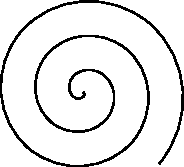
\includegraphics[width=8cm]{pics/spiral.pdf}
	\caption{A spiral... smooth vector-based with a clean parametrisation! \\ Nothing to do with \cite{Gage:18}}\label{fig:spiral}
\end{figure}
\FloatBarrier

\section{Tables}

\begin{table}[H]
	\small
	\centering
	\begin{tabular}{p{5cm}|l|p{3cm}}
		`` Industrial era '' &  ``Jobs '' & `` Wanted: Upgrade''' \\ \hline
		Parts exchanger & Fitter & mecatronics specialist \\
		eShop & reseller & `` Client-suggester'' \\
		`` Coding-guru''' & Softwaredesign & Whole-life designer \\
		JA! Gut \& Günstig & brand-names & `` Life-Style Feeling'' \\
		Internetbanking & Bank clerk & Customer adviser \\
		Robots & Specialist & Machine supervisor \\
		Bush & Gardener & Nature-sculptor \\
		Painting & Painter & Interior Design \\
		&  & \\
	\end{tabular}
	\caption[Downgrade and upgrade of job denominations]{Downgrade and Upgrade of job denominations \\ \ \ \ \cite{DueckKo:2016}}
	\label{tab:Downgrade and Upgrade of job denominations}
\end{table} 

\section{Listes}

\begin{itemize}
	\itemsep0pt
	\item one
	\item twoi
	\item threei
\end{itemize}

\begin{enumerate}
	\itemsep0pt
	\item first
	\item second
	\item third
\end{enumerate}


\section{Formulæ}

A formula can be written inline, e.g. as $ \frac{d}{dx}\mbox{arctg}(x) = \frac{1}{1+x^2}$ or, in centered math:

\begin{equation}  \frac{d}{dx}\mbox{arctg}(x) = \frac{1}{1+x^2} \label{arctanderivative}\end{equation}

Notice that formulæ that are centered start bigger (technically, they start in \verb+\displaystyle+) than they start inline (technically, they start in \verb+\textstyle+ all subsequents reductions, e.g. an exponent, goes to \verb+\scriptstyle+ then \verb+\scriptscriptstyle+). Indeed a best effort is made so that inline formulæ do not change the line height which would bother the eye of a reader.

Formulæ can be given a number and a label. Numbering happens automatically with \verb+\begin{equation}+ and \verb+\end{equation}+ and can be avoided if enclosing the formula betwee \verb+\[+ and \verb+\]+. If using the \verb+\label+ macro inside, you can refer automatically to this equation using \verb+\ref{label}+. E.g. Thanks to equation~\ref{arctanderivative} one dare say that:

\begin{equation} \int_0^t \frac{1}{1+x^2} dx = \mbox{arctan}(t) \end{equation}


\section{Tools and Code}

Many users of this template will want to include some code.

The simplest way to do so is to use the \verb+\verb+ macro which is followed by a sign, then some code, then the sign again to close. This is the inline version which works as in: 


\begin{verbatim}
	As we could calculate with \cite{Wolfram_alpha} using 
	\verb_integrate 1 / pi e ^ (t/pi) from zero to infinity_.
\end{verbatim}

which yields: 

As we could calculate with \cite{Wolfram_alpha} using \verb_integrate 1 / pi e ^ (t/pi)_ from zero to infinity.


The multiline version of this is called \verb+\begin{verbatim}+ and finishes with \verb+\end{verbatim}+.


\section{Citation examples}

Monography \citep[][S. 22]{con:infra} 

Collection \citep{sammelband} 

Article \citep{article1}

%\chapter{Conclusion}

\appendix 

% ---- Bibliography ----
%
% BibTeX users should specify bibliography style 
% References will then be sorted and formatted in the correct style.
%
 %\bibliographystyle{alpha}
\bibliographystyle{iubh}
\bibliography{biblio}

%\printbibliography[heading=none]

%\chapter{Annexes (optional)}

(with a list of them)



%\chapter{Glossary (optional)}

\chapter*{Eidesstattliche Erklärung}

\begin{figure}[t!]
	\raggedleft
	
\includegraphics[scale=0.3]{pics/logo.pdf}
\end{figure}

\thispagestyle{empty} %Seitenzahl weglassen

I hereby certify...


\vspace{1,5 cm} 
\begin{tabular}{p{7cm}p{.5cm}l}
	\dotfill \\ 
	Place, date
\end{tabular}% 
\hfill 
\begin{tabular}{p{7cm}p{.5cm}l}
	\dotfill \\ 
	Signature
\end{tabular}% 

\end{document}
